\documentclass[10pt,twocolumn]{article}

\usepackage{times}
\usepackage{fullpage}

\usepackage{booktabs}  % for \midrule
%\usepackage{subfigure}
\usepackage{balance}
\usepackage{graphicx}
\usepackage{xspace}
%\usepackage{pslatex}
%\usepackage{pifont}
%\usepackage{multirow}
%\usepackage{array}
%\usepackage{booktabs}
%\usepackage{cite}
\usepackage{url}
%\usepackage{cancel}
\usepackage{color,colortbl}
%\usepackage{microtype}
%\usepackage{textcomp}% http://ctan.org/pkg/textcomp
\usepackage{tabularx}
\usepackage{framed}
\usepackage[]{algorithm2e}
\SetAlFnt{\small}
\SetAlCapFnt{\small}
\usepackage{algorithmic}

\usepackage{listings}
%\usepackage{scrextend}
%\usepackage{mathtools}
\usepackage{pbox}

\let\labelindent\relax
\usepackage{enumitem}

\usepackage{tikz}
\usetikzlibrary{arrows,automata}
\usetikzlibrary{calc,positioning}
\usepackage{lipsum,adjustbox}

%\usepackage{tikz}
%\usepackage{decorations.pathmorphing}
%\usepackage{assymb}

\usepackage[labelfont=bf]{caption}

%\theoremstyle{plain}
\newtheorem{theorem}{\bf{Theorem}}%[section]
\newtheorem{lemma}[theorem]{\bf{Lemma}}
\newtheorem{corollary}[theorem]{\bf{Corollary}}
\newtheorem{proofl}[theorem]{\bf{Proof}}
\newtheorem{proposition}[theorem]{\bf{Proposition}}

%\theoremstyle{definition}
\newtheorem{definition}{\bf{Definition}}%[section]
\newtheorem{observation}{\bf{Observation}}%[section] 

%\theoremstyle{remark}
\newtheorem{example}{\bf{Example}}
\newtheorem{notation}{\bf{Notation}}
\newtheorem{fact}{\bf{Fact}}

\usepackage{listings}
%%\usepackage{listings-golang}
\usepackage{color}

%\usepackage{sectsty}
%\sectionfont{\fontsize{12}{15}\selectfont}


\newcommand\mypara[1]{\vspace{.3em}\noindent\textbf{#1}}
\newcommand{\urlwofont}[1]{\urlstyle{same}\url{#1}}


%%%%%%%%%%%%%%%%%%%%%%%%%%%%%%%%%%%%%%%%
% Useful reviewing/feedback annotations
\input{annotations}
%%%%%%%%%%%%%%%%%%%%%%%%%%%%%%%%%%%%%%%%


\begin{document}

\title{In-network Contention Resolution for Disaggregated Memory}
%\author{WORDS '21 Submission \#3}
\author{Stewart Grant and Alex C. Snoeren\\ UC San Diego}
\date{}

\maketitle

\section*{Abstract}

\todo{abstract}

\section{Introduction}

There has been tremendous interest in resource
disaggregation in recent years, with both academic and
industrial researchers chasing the potential for increased
scalability, power efficiency, and cost
savings~\cite{blade-server,rethinking,the-machine,requirements,clio-arxiv,firebox,leap,zombieland,storm,aifm,supernic}.
By physically separating compute from memory across a
network, it is possible to dynamically adjust hardware
resource allocations to suit changing workloads.  A large
number of
proposals~\cite{infiniswap,fastswap,legoos,clover,sherman,farm,reigons}
have leveraged the remote direct memory access (RDMA)
support found in modern network interface cards (NICs) due
to its low latency, high throughput, and simple verb-based
interface.  Yet, most share a common drawback: they do not
support sharing remote memory across compute nodes.  For
systems which do provide sharing even modest levels of write
contention crater the performance of those that attempt to
do so~\cite{clover,sherman}.

The reason behind this limitation is easy to identify: sharing remote
memory requires coordinating access across multiple clients, yet the
RDMA protocol---like TCP---provides a connection-based abstraction;
while connection-less operation is possible, much like UDP it provides
essentially no semantic guarantees.  Fundamentally, remote memory
operations must be ordered to provide coherent access, and the RDMA
protocol provides two basic mechanisms to do so remotely (i.e., in a
1-sided fashion): reliable connections that ensure ordering and atomic
operations that deliver mutual exclusion.  While the performance of
RDMA connection handling has received considerable attention~\cite{farm,storm,scalerpc},
connections remain an end-to-end abstraction, and do not provide any
guarantees regarding operations from distinct clients.  For that,
systems must rely on atomic operations like compare-and-swap (CAS),
but their enhanced semantics dictate expensive implementation choices
on the NIC, dramatically restricting their performance compared to
simple verbs like read and write~\cite{design-guidelines}.  Moreover,
atomic operations are available only over reliable connections.

As a result, most existing systems that deliver scalable,
high-performance shared remote access depend on the presence of
computational resources collocated with the remote
data~\cite{herd,cell,farm,pilaf,storm}.  In particular, a
memory-local CPU can employ 2-sided RDMA operations to orchestrate
operations between multiple clients~\cite{herd,fasst}, avoiding the need
for atomic operations.  Unfortunately, such RPC-like approaches are
infeasible in the passive memory setting.  Alternatively,
organizations with significant resources have considered redesigning
the RDMA protocol itself to better support the needs of the
disaggregated usage case---by, e.g., removing the connection
abstraction and providing more powerful verbs~\cite{filemr,rma,star}---but such
hardware is not yet available.

%% Fast
%% networks have enabled practical disaggregation for
%% non-volatile storage (SSD, HDD), as RTTs are a fraction of
%% the media access latency. In contrast practical remote main
%% memory is still on the horizon as DRAM access times remain
%% around 20x lower (1us vs 50ns) than an intra rack RTT.

In this work, we explore an alternative dimension: rather than relying
exclusively on end-to-end solutions, we consider leveraging in-network
resources---specifically programmable switches that are located between
clients and the remote memory servers---to accelerate systems based on
existing 1-sided RDMA verbs.  Concretely, we observe that in
rack-scale disaggregated settings, the top-of-rack (ToR) switch serves as a
single serialization point for all RDMA requests.  As a result, it is
possible to transparently rewrite RDMA operations in flight to
orchestrate requests from multiple clients to passive memory servers,
sidestepping the fundamental bottlenecks present in the current
connection-based RDMA protocol.


%% Resolving conflicts is hard because no centralized
%% serialization point exists. RDMA key-value stores use CPU's
%% on remote machines to serialize
%% writes~\cite{herd,cell,farm,pilaf,storm}, in the
%% disaggregated setting remote memory is not collocated with a
%% CPU, so no such serialization point exists. When clients are
%% collocated they can share an RDMA reliable connection which
%% provides in order delivery~\todo{Anil whats the RDMA
%% scheduling paper}, but in general, distributed clients
%% sharing remote memory must heavyweight RDMA atomic
%% operations to serialize requests, RDMA atomics are known to
%% not scale, and when issued by multiple clients to a shared
%% address, such as in the case of a lock, are 6x slower than
%% read/write verbs~\cite{design-guidelines}. However, at rack
%% scale, RDMA requests to remote memory are serialized, not
%% explicitly by a CPU, but implicitly when serialized on the
%% egress port of a TOR.

We present \sword, a top-of-rack switch that implements two separate
yet complimentary approaches to accelerating RDMA-based passive
memory~\cite{Grant2021InContRes}.  Client-driven schemes must rely
either on mutual exclusion (i.e., locks) or optimistic concurrency
control (which require multiple round trips to resolve conflicts).
\sword\ removes the performance bottlenecks of both by 1) multiplexing
multiple clients' RDMA operations onto shared connections to leverage
the ordering semantics delivered by reliable connections~\cite{flock},
and 2) caching small amounts of metadata to dynamically steer
in-flight RDMA updates to serialize concurrent operations to
remote-memory indexing structures.

We apply \sword\ to two existing remote memory systems which natively
support sharing: Sherman~\cite{sherman}, which uses locking, and Clover~\cite{clover} that relies on optimistic concurrency.
We show that both systems natively collapse under contention due to RDMA's
limitations, but \sword\ can remove their bottlenecks.  Concretely, 
%% We address these limitations with \sword. {\sword} resolves
%% conflicts to remote memory by interposing on, and modifying
%% in-flight RDMA requests. Small amounts of metadata are
%% cached (just enough to detect and resolve conflicts). \sword
%% requires no modifications to the existing systems to
%% provide a performance boost.  We demonstrate with Sherman
%% and Clover that both locking, and optimistic concurrency can
%% be accelerated by orders of magnitude. 
%% %%
by multiplexing all acquire and release operations for a shared lock
in Sherman onto a single reliable connection, \sword\ can
replace the client-issued compare-and-swap operations
with a lightweight writes, delivering a potential 10$\times$ gain in
throughput.  Performance gains are even higher in the case of Clover,
where
%% When access to a shared location (lock acquire, release) is
%% required we show that our middlebox can multiplex reliable
%% RDMA connections, similar to collocated requests, thus
%% removing the need for atomics entirely. Here we swap atomic
%% operations with writes for a potential 10x gain in
%% throughput. In optimistic schemes when requests are not
%% necessary destined for the same address we
we resolve update conflicts to Clover's internal, append-only metadata
index structure by steering requests to an advancing set of locations,
as if they had been issued by a single serialized client.
Our evaluation shows that
%{\sword} dramatically increases
%the performance of Clover in the presence of write
%contention: U
under a 50:50 read-write workload, throughput
rises by almost 35$\times$ while bandwidth usage and tail
latency drop by 16 and 300$\times$.


% There has been tremendous interest in resource disaggregation in
% recent years, with both academic and industrial researchers chasing
% the potential for increased scalability, power efficiency, and cost
% savings~\cite{blade-server,fastswap,rethinking,the-machine,requirements,clio-arxiv,firebox,leap,zombieland,storm,aifm,legoos,supernic}.
% By physically separating compute from storage across a network, it is
% possible to dynamically adjust hardware resource allocations to suit
% changing workloads.  Considerable headway has been made at higher
% levels of the storage hierarchy; published and even production systems
% support remoting spinning disks, SSDs, and modern non-volatile
% memory technologies~\cite{decible}.  Remote primary storage---a.k.a.
% memory pooling---remains a fundamental challenge, however, due to the
% orders-of-magnitude disparity between main-board access latency and
% even intra-rack round trips.

%Resource disaggregation is an architectural paradigm which separates
%disk, CPU and memory over a network. The goal of this architecture is
%to enable extreme flexibility in terms of machine composition.  For
%example a systems memory capacity can be dynamically apportioned by
%reconfiguration, rather than by manually changing the physical
%components of a single machine. It is now common for disks (HHD and
%SSD) to be disaggregated from CPU and memory. SSDs are comparatively
%easier to disaggregated than main memory as their access latencies are
%on the order of 10's of microseconds which amortizes the network round
%trip cost.

%Local memory latency is around 50ns. The cost of accessing memory over the
%network is on the order of 1us -- approximately a 20x overhead. This order of
%magnitude difference in latency makes hiding remote memory accesses a hard
%problem.  

% The hardware community has made great strides in closing the latency
% gap via novel technologies like silicon photonics and new rack-scale
% interconnects, but commercially available options remain significantly
% slower than on-board alternatives.  Concretely, while industrial consortia
% have proposed cache-coherent memory technologies~\cite{genz,cxl} that
% would dramatically lower access latencies, currently available
% interconnects based on RDMA~\cite{infiniband-spec}
%%
%\todo{distinguish CXL 200-500ns latencies have been proposed}
%%
% remain on the order of 20$\times$ slower than a local access (e.g.,
% 50~ns local versus 1~$\mu$s remote).  As a result, despite the fact
% that current-generation memory transport technologies provide the
% ability to directly execute requests like read, write, and compare-and
% swap-on remote host memory through the use of RDMA-capable
% NICs~\cite{connectx}, SoCs~\cite{cavium}, FPGA
% SmartNICs~\cite{corundum,kv-direct}, or DPUs~\cite{fungible}, most
% existing systems coordinate with a remote CPU on the socket at which
% the DMA is being performed to assist with
% serialization~\cite{cliquemap,erpc,herd,sonuma,storm}.
% %%


%% % and Omni-Path~\cite{omni-path}. // omni-path is dead now % 
%Each protocol, while distinct, meets approximately the same requirements,
%reliable access to byte addressable remote memory with low latency and high
%throughput.

%% it would be nice to Cite SUPERNIC and CLIO here but I'm not sure it makes
%sense untill it's published at a major venue
%%Clio~\cite{clio-arxiv}
%%todo ask alex about the archive reference
%%todo do a quick read of how DMA is dealt with on the other interconnects

% In the absence of a general-purpose CPU located alongside remote
% memory, it falls to each individual client to ensure that its reads
% and writes are serialized, usually by leveraging expensive
% hardware-provided atomic operations at the server like
% compare-and-swap (CAS)~\cite{design-guidelines} as the latencies
% involved in client-side coordination are prohibitive.  As a result,
% most existing systems simply partition memory completely and forgo
% sharing~\cite{reigons,fastswap,legoos}.
%%
%The few published systems that provide fully passive remote memory
%target scenarios involving read-heavy workloads~\cite{clover}, client
%colocation~\cite{sherman}, or memory-inefficient
%datastructures~\cite{race} \textbf{XXX:Need to say more} where the
%costs of conflict detection and resolution can be effectively
%amortized.
%
% The few published systems that do support shared access mediate
% requests to specialized data structures~\cite{clover,sherman}.

% For example, Sherman, a write-optimized
% B+Tree~\cite{sherman} places its locks in NIC memory at the server to
% avoid crossing the remote PCIe bus.
% %, resulting in 3$\times$ higher throughput.
% Clover~\cite{clover} implements a hash table that
% supports lock-less reads; concurrent writes are supported through a
% client-driven optimistic concurrency protocol.  Despite their clever
% designs, however, both approaches simply delay the inevitable:
% %%
% Sherman's NIC-based locks are subject to significant hardware limits
% imposed by the CAS operation required to enforce serialization.
% Similarly, Clover's client-based recovery scheme quickly becomes cost
% prohibitive when faced with non-trivial levels of write contention.
%
%it is repeatedly executed on a single
%address (Lock acquire and release). Further, Sherman requires that cliques of
%clients are colocated to resolve most contention based conflicts locally.
%%
% CAS instructions are only executed to commit
%writes and never land on the same address twice - effectively bypassing the
%single address limits of CAS.
%%
%While highly scalable for read-heavy workloads,  This

% We argue that these shortcomings are not unique to the particular
% systems, but rather fundamental to any approach that implements
% distributed conflict resolution.
%
%% minimize conflicts by caching  metadata about the
%% location of the latest writes and reads while also make use of a
%% remote data structures which allows for lock-less reads. In the case of
%% highly contended resources however the performance of clover
%% diminishes sharply due to an increased number of atomic locking
%% operations required on writes.
%
% The obvious alternative is to deploy a centralized memory controller
% (e.g., a CXL 2.0 switch) that can serve as a serialization point and
% ensure all races are resolved before accessing memory, but effective
% realization of such a design has proven elusive.  While many proposals
% exist, none of them have yet been implemented in commercially
% available hardware.  More to the point, such designs are inherently
% unscalable as they require all accesses to be managed by the
% controller, rather than forwarded directly between the client and
% relevant server.

% In this work we make the observation that such a serialization point
% already exists in today's rack-scale disaggregated deployments: the
% top-of-rack switch.  We propose to leverage the capabilities of modern
% programmable switches to cache sufficient information about in-flight
% requests to transparently detect and resolve conflicts before they
% occur.  Unlike a centralized memory controller, however,
% our serializer does not need to operate on---or even maintain state for---all
% remote memory requests.  First, it only needs to address actual conflicts
% and can avoid the unnecessary costs of enforcing ordering among
% unrelated requests.  Second, in deployment scenarios where it may
% lack the resources to track all requests, our serializer can serve as a
% performance-enhancing proxy: when deployed alongside client-based
% conflict resolution techniques, it can allow even conflicting requests
% to pass through unmodified without jeopardizing safety while
% decreasing the frequency of conflict resolution.

% We present {\sword}, an on-path serializer
%(implemented either
%directly on the top-of-rack switch or an attached
%middle box~\cite{disandapp})
% that dramatically improves the performance of remote memory systems
% that support write sharing.  Like all ToRs, {\sword} imposes a
% globally observable total order on memory requests (i.e., packets)
% within a rack.  In scenarios where {\sword} has the resources to
% explicitly manage RDMA connections, it can enforce per-server ordering
% at the ToR and remove the expensive CAS operations from all in-flight
% packets, avoiding their associated performance bottlenecks entirely.
% More generally, however, {\sword} can be deployed alongside an
% underlying optimistic concurrency scheme: remote memory operations
% remain guarded to ensure that clients can detect and recover from
% conflicts of which {\sword} may not be aware.  Instead, because
% {\sword} understands the disaggregated memory protocol, it can keep a
% cache of recent operations to adjust subsequent requests whose
% guards it knows are doomed to fail.  In such cases,
% %If suitably provisioned (i.e., it has the
% %appropriate metadata cached),
% it modifies requests in
% flight to account for the preceding operations and decrease the
% likelihood the guard will trip.

% We prototype {\sword} in two scenarios using a rack of servers
% equipped with ConnectX-5 RoCE-enabled NICs.  First, we use a
% DPDK-based implementation to replace CAS requests in flight with
% standard RDMA verbs, allowing systems like Sherman to overcome the
% hardware limit on atomic requests per queue pair.  Second, we
% implement a lightweight version of \sword\ on a P4 programmable switch
% to accelerate Clover's optimistic concurrency protocol. Our evaluation
% shows that {\sword} dramatically increases the performance of Clover
% in the presence of write contention: Under a 50:50 read-write
% workload, throughput rises by almost 35$\times$ while bandwidth usage and tail latency drop by 16 and 300$\times$.

% %% Using RDMA transport information and clover specific application
% %% knowledge all reads and writes to contended areas are totally ordered
% %% in the network. Specifically all reads and writes to the same keys are
% %% multiplexed to the same queue pairs, by utilizing the RDMA ordering
% %% requirements of QP's reads and writes require no expensive locks and
% %% can flow at line rate to remote memory. This ordering requires a
% %% number in band adjustments to the RDMA protocol in order to
% %% interoperable with commodity hardware. QP state must be maintained in
% %% network, specifically the sequence numbers of multiplexed requests, so
% %% that response packets can be demultiplexes back to their original
% %% connections. Small adjustments such as generating ACKs for collapsed
% %% requests is also required. We demonstrate that these algorithms are
% %% implementable in network at little cost with a DPDK prototype. We
% %% measure that ~\todo{we achieve a ?X improvement in performance using
% %%   only XMB of in network state, and ?X performance improvement in
% %%   highly contested settings with full use of system memory}.

\section{Background}

While our insight and approach is general, in order to demonstrate its
practicality we prototype it in the context of Clover~\cite{clover}, a
disaggregated key/value store.  Hence, we begin with a brief overview
of the relevant aspects of Clover's design for the uninitiated.

\subsection{Append-only updates}

Clover maximizes read performance by separating key/value metadata
from the datapath, which is implemented as a linked list of value
updates that the authors term a \emph{chain} that supports an atomic
append-to-tail operation.  Each value update contains a pointer to the
next update in the version chain, and metadata servers keep pointers
to the current tail of the chain for each key allowing clients to
issue lock-free RDMA reads directly to passive remote memory servers
using the address they believe to be the current end of the chain.
Clients can independently confirm their reads are fresh by ensuring the
value returned has a ``null'' next-update pointer.

Write (i.e., append-to-tail) operations, on the other hand, require
multiple steps.  First a writer issues a lock-free RDMA write to store
the new value update in an uncontended portion of remote
memory. After the RDMA operation completes a second operation
optimistically attempts to atomically add the new update to the end of
the chain.  Specifically, the writer issues an RDMA compare-and-swap
(c\&s) operation to the old tail to replace its (presumably still
``null'') next-update pointer with the address of the new value.  If
successful the client lazily updates the metadata sever with the
new end-of-chain address.
%(as any concurrent writes to the
%same location will fail the comparison).

%% This operation ensures that the next
%% write to the data structure writes to the tail of the linked list.
%% This operation requires two steps.

The authors show their opportunistic approach obtains extremely high
throughput with read-heavy workloads as updates are rare and clients
enjoy unfettered access to remote memory. In contrast they find that
placing a metadata coordinator on the datapath becomes a bottleneck at
only a fraction of their achievable throughput.  In the presence of
writes, however, Clover's throughput decreases due to contention.

\subsection{Conflict handling}

If multiple clients attempt to update the value concurrently, each
will succeed in writing their new value to remote memory but then
issue conflicting RDMA c\&s operations to the end of the chain.  The
race is resolved at the remote memory location of the previous update
in the chain: only the first c\&s operation will succeed; all
subsequent operations will fail because rather than finding a value
with a ``null'' next-update pointer, they find the now (at best)
penultimate value in the chain which points to the update issued by
the client that won the race.
%When
%concurrent writes update the same key a race occurs to write at the
%end of the chain. Write operations require two separate RDMA
%transactions that must each complete to ensure atomicity.
During this
two-RTT operation any concurrent write to the same key will cause a
conflict.

%% The process which lost the race now needs to engage in \textit{Pointer
%% chasing} to find the new tail. It must iterative issue reads of the
%% linked list, step by step until it finds the location of the new tail.


If a client's write---or read---fails because it did not succeed in
accessing the current end of the chain they concurrently request the
new address from the metadata server and traverse the chain themselves
through remote memory to find the current end in a processes known as
\emph{chain walking}.  (It is insufficient to just consult the
metadata server because they are updated lazily.)  Failed writers must
then issue a new c\&s operation at the updated end of the chain to append
their pending update.  Of course, the reissued c\&s is subject to the
same race condition as many writers may be executing
concurrently. This pointer-chasing reconciliation algorithm must be
run independently each time a conflict occurs.
%The slower writers will fail the guard, and must retry
%their c\&s operation after walking the chain through remote memory or
%by getting an update from the metadata server.
While concurrent read operations will not prevent a write from
succeeding, a reader that loses the race with a c\&s operation will
need to issue another RDMA read to the new address to obtain the
updated value.  On write-heavy workloads these race conditions happen
frequently as illustrated in Figure~\ref{fig:conflicts},
%, which leads to a sharp decrease in throughput.  For highly
%contested structures, the number of retries can grow quickly,
leading to large and unpredictable tail latencies.




\begin{figure}
    \includegraphics[width=0.45\textwidth]{fig/write_conflicts.pdf}
    \caption{Clover write conflicts grow with the number of clients
    (50\% write Zipf 0.99 distribution)\todo{redo with 64 cores and
    writes only}}
    \label{fig:conflicts}
    \vskip -0.5em
\end{figure}



%% The high level pitch about remote memory.
%Far memory projects typically have a remote CPU which is used to
%coordinate access to remote resources (cite all object systems). In a
%disaggregated system there is no remote CPU, therefore the coordination
%of reads and writes to remote locations must be done locally. For
%performance local caches of remote resources can be used to organize
%access to remote resources. For data structures which require
%consistency this creates a problem as stale caches can lead to data
%structure corruption.


\section{Benefits of on-path serialization}

Given the overhead of atomic RDMA operations and the performance bottlenecks
associated with individual queue pairs, this section considers the opportunities
made available by an on-path serializer.  In particular, if we ensure that data
races cannot arise, we can replace expensive compare-and-swap operations with
simple write verbs and use the ordering guarantees of RDMA reliable connections
to provide serializablity. Moreover with information about stateful dependencies
we can assign independent operations across multiple QP to improve scalability.

\subsection{Atomic replacement} 

In many disaggregated systems operation serialization is performed using RDMA
atomic operations implemented on a NIC. These atomics are expensive because they
can block many concurrent RDMA operations while they execute and require scarce
NIC resources. The time required to complete an atomic is at minimum a PCIe
round trip from the NIC to main memory, during which time a lock on the NIC
guards the memory access. Lock implementation is both vendor and transport
specific~\cite{design-guidelines}. In the worst case a barrier is placed on all
operations resulting in complete head-of-line blocking, in the best case locking
is per connection and only causes other operations to block when reads or writes
occur on overlapping ranges virtual memory. Regardless of the implementation
atomic operations are significantly slower than asynchronous non-blocking reads
and writes.

Because of their cost, we would like to replace atomic writes such as compare
and swap (CAS) with non-blocking writes.  From a RoCE v2 perspective the per
packet transformation from CAS to write can be applied easily in the datapath.
RoCE v2 CAS and write headers only differ by a few fields. CAS can be thought of
as a special case of a write, where the write is conditional and the length is
preset to 8 bytes.
%%
CAS packets are transformed to writes by modifying their headers. We switch the
RDMA OP field of the CAS to WRITE, copy the CAS value to the write payload
location, set the DMA length of the write to 8, and shrink the IPV4 length by 4.
Post modification the RoCE v2 and IPv4 checksums are recalculated so the
modified packet will not be rejected by the memory side NIC. The transformation
from CAS to write is deterministic and only requires a few cycles to transform
the header.

On the memory server, the NIC processes the modified CAS as a WRITE and responds
with an ACK. Once the ACK reaches our middlebox we apply the inverse
transformation from the ACK to an Atomic ACK which the sender expects to see.
RDMA Atomic ACK headers are very similar to regular ACKs with the only
difference being that the atomic contains the original data from the memory
location of the CAS. This original data is missing due to the transformation so
we inject a value which indicates success to the sender.
%%
This value is application specific; in Clover's case 64 zero bits indicate
success. Transforming CAS to write does nothing to disturb the RDMA protocol, as
both the sender and receiver side NIC are oblivious.  However, the guarantees
the atomic provides, such as write serialization and the prevention of read
tearing has been lost. To prevent arbitrary corruption of data the serialization
point must be placed somewhere else. Our approach is to detect conflicts in
network, and utilize the in order delivery guarantees of RDMA reliable
connections to ensure safe and serialized operations.

\subsection{Connection remapping}

RDMA operations made on a reliable connection (one server one client queue pair)
are guaranteed to be executed in the same order as their sequence numbers
similar to TCP transport ordering~\cite{infiniband-spec}~\footnote{while IB
allows for relaxed ordering here we rely on that feature being turned off on the
receiver}. That is operations on a single stream are totally ordered with
respect to one another. This is not true across multiple connections in the
where writes to shared state can easily corrupt one another, and reads can be
torn without the use of locks.  Our insight is that if all operations across all
connections which share state are steered to the same connection the default
RDMA ordering mechanism will provide serialization.  The determination of which
operations share state is application specific. It requires inspecting each
packet, extracting the relevant pieces of meta data, and steering the packet to
the correct connection. Here we focus on the example of Clover where requests to
read and write the same key are shared state operations.

%%While removing locking operations is a general principle here we consider a
%%solution for RDMA.  %Different transports with different ordering guarantees
%%would require bespoke solutions.  

\subsubsection{Sequence-space stitching}

Multiplexing and demultiplexing RDMA operations across established connections
requires a significant amount of care. Requests on a single connection must have
monotonic sequence numbers from the senders and receivers perspectives. If
monotonicity is broken, the NIC will invoke an expensive go-back-n protocol or
issue explicit congestion notifications. To achieve monotonic sequence numbers
on shared connections we track a sequence number per memory QP and inject the
updated sequence number into the packet after a state based mapping decision has
been made.
%%
This monotonic sequence number increment and QP maping is the serialization
point which replaces the use of the RDMA CAS operation. As long as a packet is
given an atomically incremental sequence number from our middlebox and placed on
a stateful partitioned connection, it will execute in the same serialized order
as if it were protected by a CAS. We are guaranteed this due to the ordering
requirements of RDMA reliable connections.

Once sent a stub for each mapped request is stored on the middlebox to aid in
mapping the request back. The stub keeps track of the original requests sequence
number, IP address, MAC address, and queue pair. Stubs are stored in an array
based on their sequence number \% $table size$ for an O(1) lookup when they are
demultiplexed back to their original connections.
%%
In addition to sequence numbers, a \textit{message sequence number}, is used as
an RDMA optimization by the memory side NIC. This value is transmitted as part
of the RoCE BTH+ header in the response. It's value corresponds to the highest
request number the receiver has processed. If this value is wrong in the
response packet from the perspective of the sender, the packet is retransmitted.
We calculate the message sequence number a sender expects to see by counting the
number of operations a sender has issued and adding it to the value of the
original message sequence number for that connection.

\subsubsection{Instruction coalescing} RoCE coalesces some ACKs as an optimization.
Multiple writes can be acknowledged by a single acknowledgment, in the form of
either an ACK, ATOMIC ACK, or Read Response. This occurs when multiple RDMA
request are processed concurrently. When mapping requests, some acknowledgments
may be coalesced which are required from the senders perspective.

A final additional challenge in mapping
requests, is that receiving NICs can coalesce acknowledgement messages. Given a
single connection, if two concurrent writes are issued, it is perfectly valid
for an RDMA NIC to only ack the second write. This is a challange when mapping
requests as a coalesed message might have been for a different sender. In our
scheme as all requests have mapping stubs stored in the middle box, when a
request is coalessed a gap in the sequence number is observable. In this case we
generate the coalesed request. While read, and CAS requests can not be
coalessed, CAS requests mapped to writes can be. In the case of coalesed ATOMIC
acks an atomic ACK is generated in place of the coalessed write ack.

\section{Improving Clover performance}

To quantify the potential performacne gains an on-path serializer can
realize in practice, we apply each of the two optimizations above in
the context of Clover, a high-performance far memory system.

\todo{High level overview of system}

\begin{figure}
    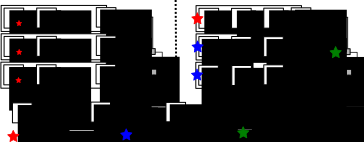
\includegraphics[width=0.45\textwidth]{fig/overview.pdf}
%%
    \caption{ System overview, Metadata, client, and Remote Memory
    servers are Clover components. Our remote memory coordinator is
    located on a centralized TOR interconnecting the clover components.
    }
%%
    \label{fig:overview} 
\end{figure}

\begin{figure}
    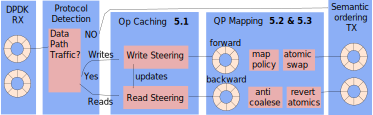
\includegraphics[width=0.45\textwidth]{fig/packet_processing.pdf}
    \caption{Our packet processing pipeline}
    \label{fig:system}
\end{figure}


\subsection{Operation Caching}
\label{sec:operation-caching}

Any asynchronous data structure which allows for lockless reads and writes must
have a mechanism in place to resolve conflicts. When memory is close, conflict
resolution strategies can make many reads and writes quickly in the uncommon
case of a conflict, the cost of which is typically amortized by the unlikelihood
of the conflict itself. In the case of far memory the cost of a conflict is
severe. In contrast to opportunistic algorithms in a shared cache architecture,
in a disaggregated system with small amounts of in network compute conflicts can
be detected and resolved in the data path. Our solution is to provide a general
framework in which developers with knowledge of their remote structures can
resolve their conflicts in network as the operations flow by serially to memory. 

\begin{figure}
    \includegraphics[width=0.45\textwidth]{fig/throughput.pdf}
    \caption{Default Clover throughput vs. Clover with write conflict
    detection and correction turned on \todo{recompute with the read caching values (old)}}
    \label{fig:throughput}
    \vskip -1em
\end{figure}

\subsection{Implementing Atomic replacement}

In the
following subsections we describe the dangers of removing atomics, and present
our solutions.

A few assumptions must be made in order for this replacement of operations to be
made. First and foremost all operation serialization must be made, and finalized
at the point where the CAS is swapped out. More formally, all of the data
structure invariants which required locking, must be satisfied at the time of
transforming the packet. Further the order of operations must be maintained
downstream from the checking of the invariant. These two requirements influence
the design of any system which aims to make this performance improvement.

\textbf{writes:} In the case of clover we cache the location of the latest writes to occur for
each key. If a write occurs which is for a stale virtual address, our conflict
detection algorithm first uses information about clovers algorithm to find the
value of the key in each RDMA write packet. We find this value by checking the
size of the write, and checking the location in the packet for specific clover
data. Once the key from the write is extracted a table lookup is used to
translate the key into the virtual address of the latest write for that key.
This strategy uses 64 bytes per key, as each RDMA virtual address is 64 bytes.
By performing this lookup in the data path all writes succeed regardless of how
contested the memory address is. \todo{ref fig from words}.

\textbf{reads:} Reads present a slightly more complicated case. Writes contain
the key, which allows for a table lookup, while RDMA read requests only contain
a virtual address and a size. When a read fails it must be retried, as mentioned
earlier reads are performed iteratively until the tail of the list is reached,
which in the case of highly contested keys could be arbitrarily long. Repeating
reads does not destroy system performance as they are lockless, however in terms
of client latency each retry adds serious latency. What makes handling reads
hard is identifying the clover key for which the read is for, without additional
data in the packet the value must be determined another way. As reads can be for
arbitrarily old virtual addresses a naieve solution would be to store the entire
lineage of each key, which would require caching all of clovers meta data in the
network. Our solution is to hash the address of each write into an array
~\todo{2x} the size of the keyspace. When writes occur their virtual address and
key value are stored in the array. New writes simply overwrite old values in the
table. This allows keys with higher hit rates to maintain longer histories in
the table. When reads occur their address is looked up in the table, if the
address has a hit the read is steered to the tail of the list. If a miss occurs
the read is left to flow through, clovers default mechanism kicks in and
performs a lookup to the meta data server for the last known address and the
process repeats. We found that by using an array size of 8x the ~\todo{vast
majority of reads succeed first try.} While the number of reads that require a
second try is ~\todo{a number}. ~\todo{insert the CDF of read retries}.

%% ACS - This is just lifted from WORDS; no need to repeat here

%% \begin{figure}
%%     \includegraphics[width=0.45\textwidth]{fig/cache.pdf}
%%     \caption{Performance as a function of keys cached. Caching a few
%%     of the top-$N$ keys provides the greatest marginal throughput
%%     benefits.}
%%     \label{fig:cache}
%% \end{figure}

%% \textbf{reduced cache size} we show that if hot keys are known we require only a
%% small amount of in network state~\ref{fig:cache} we have considered dynamic
%% approaches such as LRU which would allows for a finite amount of space and an
%% arbitrary number of keys to be serviced.

 

\textbf{1) metadata required} The first requirement, that the structural invariants
of the data structure be maintained at the point of transformation demands that
all of the state required to check the structural invariant be present at the
point in the network at which the swap is made. This fact increases the memory
cost on a switch, however with intelligent data structure design the cost of the
required metadata can be mitigated. In the case of Clover, while each key has
an entire linked list history that can potentially span megabytes, the only
required metadata to make the change from CAS to write is the location of the
tail pointer. In this case the metadata cost is O(n) as it grows linearly with
the keyspace.

\textbf{2) reordering} The second requirement, that operations not be reordered
after the invariant has been checked requires more care in real systems. For
instance in an RDMA system with two clients, both could have contesting CAS
operations swapped with writes. As the two clients are transmitting operations on
separate QP, and the receiving NIC makes no guarantees about ordering between QP,
the operations could easily be reordered. In the case with CAS, the order could
be forced by ensuring that if one write was to succeed the second would fail.
Without this guarantee the preservation of operation ordering must be maintained
in another way.

\subsection{Connection Remapping}


Our solution here is simple, given that we have the key's for reads and writes
(Section ~\ref{sec:operation-caching}), all operations for the same key are
mapped to the same QP.  This algorithm requires that a few pieces of state be
maintained per connection.  First the sending and response QP for each sender
and receiver need to be tracked. Second the sequence number of each connection,
and the original message sequence number offset must be maintained. Per client
connection the pair of QP's require 48 bits, and the sequence + message sequence
require an additional 48 for a total of 12 bytes per connection. The storage
requirement for mapped requests varies based on the algorithm. If clients are
able to issue an unbounded number of async requests, then a buffer large enough
to maintain backwards mappings for each request is required. In clover clients
can issue up to 2 async requests, so we keep a two 6 byte mappings for each
connection available to map back. 

Depending on the algorithm and the QP mapping scheme requests from a single
sender can be reordered. That is, if a client makes a read and write request to
different locations in memory, and they are mapped to different QP, they may be
returned out of order. Infiniband allows for out of order operations on
receivers~\cite{infiniband-spec}, which pushes operation ordering to client
side user space. Roce does not allow for out of order operations. In this case
the receiving NIC will retransmit if requests are delivered out of order. Here
we buffer requests in network, as we have application knowledge the size of the
buffer is bounded (to the size of a single read packet in clovers case). We
suggest that given the tight memory restrictions on middleboxes algorithms which
have an unbounded number of async requests leave the ordering of remapped
requests to client side user space using IB verbs or a different transport layer
entirely.

\todo{these sections may not be nessisary}

\subsection{Traffic Identification} Depending on the design of a disaggregated
rack memory traffic might be coresident with regular network traffic.
Additionally some of the traffic on the memory bus may not require tracking or
manipulation. In the case of clover we do not modify any traffic to the metadata
server as it is not in the read/write path. The first stage of our packet
processing pipeline is to match requests for manipulation. In our design users
submit a filter as part of their program to allow traffic which does not need to
be modified to flow freely.

\subsection{Dynamic enable/disable of connections, and epochs} A key goal in our
design is to not require the existence of a middle box in the data structures
algorithm. Clover for instance is designed to deal with memory operations made
to the wrong location via iterative pointer chasing. We strongly suggest that
disaggregated algorithms take this approach as our middlebox solution only acts
to acclerate operations in the common case. We add and subtract connections
based on the send and receipt of a single CAS operation. The QP and sequence
number for the CAS are stored on send, and the ATOMIC ACK is used to retreive
the other recevers QP. As this approach requires only a single packet requests
can be added and removed from our algorithm dynamically with little effort. As
some state may be dependent on the number of connections (such as the key to QP
mappings), state transitions either require a lock, or the coping of current
state over to a new epoch when new connections are added. In all of our
experiments only one such transition is made. We begin our mapping after a
specific number of clients for the experiment have connected. Once the total
number of clients have connected, a switch is flipped, and the QP multiplexing
algorithm begins. Requests which do not have mappings stored, but were in flight
during the flip have their sequence numbers, and MSN values applied to the
connection state of the new epoch.


\section{Evaluation}
\label{s:results}

Adding computation to the network increases latency and consumes memory. Our
evaluation demonstrates that by applying our techniques we are able to see
significant performance boosts in terms of overall throughput, and latency for
existing systems. We discuss the memory implications and show that systems
performance can be significantly improved by replacing compare and swap
operations with writes.

\subsection{Testbed}

Our testbed consists of five machines: a Clover memory server, metadata server,
and two Clover clients; the last machine hosts {\sword}. Physically, the
machines are identical: each is equipped with two Intel Xeon E5-2640 CPUs and
256 GB of main memory evenly spread across the NUMA domains. Each server is
equipped with a Mellanox ConnectX-5 100-Gbps NIC installed in a 16x PCIe slot,
all of which are connected to a 100-Gbps Mellanox Onyx Switch. All Clover
servers are configured with default routing settings: clients send directly to
the metadata and data servers. We install OpenFlow rules on the Onyx switch to
redirect the Clover RDMA traffic to \sword; Figure~\ref{fig:overview} shows the
layout of our testbed.

\subsection{YCSB benchmarks}

\begin{figure*}
    \includegraphics[width=1.0\textwidth]{fig/full_system_performance.pdf}

    \caption{{Performance of {\sword} techniques applied to Clover on YCSB
    benchmarks. The percentage of workload writes increases from left to
    right.}}

    \label{fig:full_system_performance}
\end{figure*}

The YCSB benchmark consists of varying read and write workloads which
have been shown to emulate many common datacenter
operations~\cite{ycsb}. We show how \sword's read and write steering
improve the
%a
%breakdown of our techniques, mainly read and write caching, QP mapping, and
%atomic replacement with respect to their effect to system
performance on two
YCSB benchmarks. We choose YCSB-B (95\% read and 5\% write) as our baseline, and
YCSB-A (50\% read and 50\% write) to demonstrate how our algorithm performs
under high contention.  We also show the performance boosts obtained while
running a 100\% write workload which is intended to emulate other programmatic
workloads which are update heavy.

Figure~\ref{fig:full_system_performance} shows the relative
performance gains from each of \sword's techniques. At 5\% reads write
steering provides minimal performance improvement as the vast majority
of writes succeed on their first try. Individual writes, however, can
lead to many stale reads immediately thereafter which leads write steering
to offer a 1.17$\times$ throughput improvement.
%
%Applying QP mapping to the
%read majorly case adds too much computational overhead to give a
%benefit when writes are low, and only a few compare and swap
%operations exist.
%
At 50\% writes, Clover is well outside of it target workload:
at 64 threads, over half of all write operations fail. Here applying write
steering improves performance by over 1.73$\times$ at 64 threads.

Write steering alone is not sufficient at this level of contention,
however.  Because all writes succeed they easily out-pace reads causing
the majority of reads to fail at 64 threads.  (The resulting impact on
tail latency is clearly shown in Figure~\ref{fig:tail_latency}.)
Applying both read and write steering, on the other hand, yields a
2.82$\times$ throughput improvement as nearly all operations
succeed.

%This workload leads to enough common case failures that
%performance overhead of performing QP mapping still yields a
%performance boost.

Write-only workloads are antagonistic for Clover's optimistic
approach.  Write-only and write+read steering yield 3.89$\times$ and
3.63$\times$ throughput improvements respectively; the read steering
logic is pure overhead due to the complete lack of reads in the
workload.



%%\todo{real takeaways}

% \subsection{Memory Utilization}
% Our techniques give a performance boost at the cost of in network memory. We
% took special care to design our algorithms so that they could 1) use only a
% small amount of network memory, 2) be scalable depending on the resources
% available. We show how our performance varies as a function of the available in
% network state.

% As seen in Figure~\ref{fig:cache} our write caching is able to provide a
% significant performance boost while only using a small number of cached
% addresses. In the following experiment we show the maximum performance boost we
% can provide as a function of the available in network memory. Specifically in
% the case of read and write caching this means shrinking the size of the
% available cache. In terms of QP mapping it restricts the number of connections
% which can have their connections mapped. Unmapped connections must use atomic
% operations for their requests to succeed.

% \begin{figure}
%     \includegraphics[width=0.45\textwidth]{fig/memory_util.jpg}
%     \caption{{Relative performance improvement of our techniques with restricted amounts of memory. Here a rightsized allocation implies that for the given number of connections we could support, all requests were mapped and reads and writes were cached.}}
%     \label{fig:memory_util}
% \end{figure}
%%\todo{say something real about the the memory utilization takeaways}


\subsection{Bandwidth reduction}

\begin{figure}
    \includegraphics[width=0.5\textwidth]{fig/bandwidth_reduction.pdf}
    \caption{Bytes required per operation for each of the three techniques for different write intensities.}
    \label{fig:bandwidth_reduction}
\end{figure}

Placing memory operations in-band with regular network traffic can be
problematic as applications' remote memory usage has the potential to
vary dramatically per application.  Under contention, memory operation
can require additional packet exchanges which inflate the bandwidth
necessary to service the same number of memory requests. Our
in-network steering algorithms remove the need for operations to
retry.

%Figure~\ref{fig:bandwidth_reduction} shows the average bytes
%per Clover operation under three different workloads for default
%Clover as well as {\sword}'s two steering techniques.

We calculate the optimal expected cost of a Clover operation by
averaging the cost of a successful operation across reads and
writes. We get the weighted average by multiplying the cost of a read
and write by the appropriate workload percentage. Each write consists
of an RDMA write followed by a CAS, along with the responses for each
message. A read consists of an RDMA read and read response, and
usually an additional metadata read made asynchronously with the main
read to fetch the latest position of the tail in case the first memory
read fails. Clover performs this second read opportunistically (in
around 99 percent of all reads in these workloads), however sometimes
it is omitted leading to a small over-approximation in our estimate of
``optimal''.

Figure~\ref{fig:bandwidth_reduction} show the average bytes per
operation for each strategy across all three write workloads. We
calculate the value for each technique by summing the total bandwidth
across a run and dividing by the total number of operations. Clover's
bandwidth usage increases with contention, growing by 1.8$\times$ at
50\% and 2.24$\times$ at 100\% writes---all of which is recovered by
applying read and write steering. Write steering alone causes
significant inflation in the cost of operations at 50\% writes because many
read operations fail as discussed above.

\subsection{Tail latency}

\begin{figure*}
    \includegraphics[width=1.0\textwidth]{fig/99th_latency.pdf}

    \caption{Left: Read tail latencies 99th percentile. Right: Write latencies.
    Each measure taken on a Zipf distribution of requests with 64 clients. Note that the y axis is log scale}

    \label{fig:tail_latency}
\end{figure*}

Perhaps the most critical variable that governs overall system
performance is tail latency. In the context of disaggregated memory
systems, reads and writes are often deeply integrated into the
computational logic of a program and the whole program must wait for a
page fault to complete before continuing. We therefore consider poor
tail latency to be a fundamental barrier to the widespread adoption of
far memory systems.  Optimistic concurrency is well known to exhibit
poor tail latency under contention, and Clover is no exception to this
rule. Our techniques significantly reduce tail latency as steering
ensures that nearly all operations succeed with no need to retry.

Figure~\ref{fig:tail_latency} shows the 99th-percentile tail latencies
associated with each of \sword's techniques in comparison with default
Clover. Clover's read latency (left-hand plot) at 5\% reads is
91~$\mu$s, around 7.5$\times$ its baseline our our testbed. With read
and write steering the tail latency of reads drops to 38~$\mu$s---a
2.3$\times$ improvement over Clover even in this low-contention
regime. At 50\% writes the performance increase is roughly double.  As
discussed above, in either case applying write steering alone actually
hurts performance, as it makes reads more likely to fail.
%read performance is improves by 2$\times$
%relative to Clover with the exception of write steering alone. When
%write steering is applied without the aid of read steering the writes
%quickly out-pace the reads, leading the vast majority of reads to fail
%on their first attempt.
Given that these tests were conducted with a
Zipf distribution across 64 cores it is highly likely that more than
one thread is writing to the hottest keys at any point during the
run. This leads some read operations to fail 10s of times before
succeeding.

%Because of this property we suggest
%that read and write steering be used in concert unless the workload is
%explicitly known.

Writes (right-hand side of Figure~\ref{fig:tail_latency}) perform
worse than reads under contention in default Clover. Write+read
steering provides a 2.7$\times$, 37.1$\times$, and 25.2$\times$
improvement in tail latency, respectively, across 5, 50, and 100\%
write workloads.  As one might expect, performing write steering alone
privledges writes over reads, dropping their tail latencies even
further---but likely insufficiently enough to make up for the dramatic
spike in read tail latency

Figure~\ref{fig:tail_latency} also shows the performance of queue pair
mapping and atomic replacement (CAS$\rightarrow$Write) when applied in addition
to write+read steering.  Because the operations are already likely to
succeed, there is no reason to expect any significant drop in tail
latency by vectoring the operations to a particular QP or removing the
CAS guard.  Rather, these plots show that the (significant) additional
logic required in {\sword} to implement these functions result in only
marginal increase in tail latency relative to steering alone---and still
significantly outperforms default Clover.

%The application of QP mapping and swapping
%CNS to writes does little to effect tail latency as their performance
%cost comes largely as an increase to the average.


\subsection{Atomic replacement}

\begin{figure}
    \includegraphics[width=0.5\textwidth]{fig/cas_vs_swap.pdf}
    \caption{Throughput of conflicting CAS and rewritten CAS operations as a function of client threads/QPs.}
    \label{fig:cas_vs_swap}
\end{figure}

We show the ability of swapping compare and swap operations to writes
to overcome hardware atomic bottlenecks by running a micro-benchmark
that focuses exclusively on CAS performance.  Specifically, we extract
the CAS request alone from Clover's write operation (recall it
consists of both an RDMA write and CAS) and repeatedly generate it
from one client to a single memory server (while routing it through
{\sword} as before).

%Here we remove clover from the
%mix and run a simple benchmark of RDMA CAS operations between two
%servers. \sword is routed to via a different set of OpenFlow rules.

Each client thread is bound to a its own queue pair, and all client
threads issue CAS operations to the same shared virtual address.  We
set the number of cores on the {\sword} middlebox to 24 so that in our maximal
test case each client thread flows through exactly one middlebox core
for the lowest degree of interference between QP.

%All requests are routed
%through our middlebox.
In the default case (labeled CAS in Figure~\ref{fig:cas_vs_swap}),
{\sword} lets CAS operations flow through without interference, each
on their own queue pair.  In the CAS$\rightarrow$Write configuration
{\sword} needs to rely upon the ordering semantics of RCs (because all
the operations are for the same memory address and therefore
conflict), so maps all client requests to the same QP at the server.
Due to DPDK queue-to-core partitioning requirements all TX for a
destination QP must be done by a specific core on the
middlebox. Because of this requirement all requests in this
configuration must flow through a single core prior to being issued to
the memory-side NIC.

%all client cores request the same address, and as such all are routed
%onto the same destination QP. Note that this configuration has the
%highest degree of contention for our middlebox as 24 client threads
%must be multiplexed to and from a single client connection. Further

We measure the server throughput in terms of operations per second as
we increase contention by adding client threads.
Figure~\ref{fig:cas_vs_swap} shows the performance gained by
converting CAS operations to writes. Both configurations hit distinct
bottlenecks: CAS operations bottleneck due to being applied to a
single key (c.f. Figure~\ref{fig:rdma_concur}). In the case of
converting CAS to write, the bottleneck is the processing power of the
CPU cores in our DPDK-based {\sword} prototype. (The maximum throughput
our prototype can process is 2.8 million operations per second per
core.)
%In this configuration all
%requests to the memory server must be processed by the same TX
%core. As such our bottleneck is approximately 2.8 MOPS. Hardware
%implemented CRC, cache tuning, and better lock management for TX
%queues could yield higher per core performance in the future.
Despite this implementation restriction, these results clearly show that
replacing CAS with write avoids the memory server NIC's hardware
bottleneck, enabling increased scalability with a more performant
{\sword}---such as one implemented on a programmable switch.

%\section{Abstract}
\todo{the whole thing :(}

\section{Intro}
\label{sec:intro}

%%State of the world
Disaggregated computing promises higher resource density, increased
power-efficiency, and flexible application scalability in datacenters.
While enticing, these benefits have remained mostly untapped due to
the proportionally large overhead of accessing remote resources.
Nowhere is this disparity more noticeable than remote memory.
Separating CPUs last level cache from their main memory incurs at
least a 20x overhead (approximately 50\textit{ns} to 1\textit{us}).
The cost is only acceptable for select asynchronous workloads, such as
paging out infrequently touched data~\cite{infiniswap,legoos,leap},
but are entirely unrealistic when multiple CPUs require consistency
for frequent reads and writes to shared remote memory.

A large body of work has investigated how to design high performance
RDMA key value stores, and RPC
frameworks~\cite{cell,sonuma,storm,farm,herd,erpc}. However, they
require that a CPU be coresident with remote memory to coordinate RDMA
access and keep their remote data structures consistent. In the case
of pure resource disaggregation no CPUs are coresident with remote
memory. This architectural difference requires new techniques and
algorithms to achieve similar functionality and performance. 

Some research has been done into the requirements for resource
disaggregation, specifically with regard to network, and memory
requirements~\cite{requirements, aguilera2019designing, disandapp,
amanda-hotnets}. Few have been tested practically and some require
non-existent hardware primitives. Those that have been constructed are
first attempts at exposing remote memory to clients without the
expectation of remote CPUs~\cite{reigons, clover}. Both Remote
Regions~\cite{reigons} and Clover~\cite{clover} are designed to use
remote memory with a read heavy workload on any shared resources.
%%
Their reason for avoiding writes is fundamental: concurrent consistent
writes to remote memory are expensive. Lock acquisition and revocation
requires multiple round trips which devastates throughput.  Even with
an intelligent concurrent algorithm to opportunistically avoid lock
acquisition the problem is pervasive due to the natural concurrency
and relatively high latency of remote memory.
%%
In the opportunistic case write conflicts due to inconsistencies in
local caches occur frequently when resources are contested.
Figure~\ref{fig:conflicts} shows the number of concurrent conflicting
writes to shared resources as the number of clients requesting the
resources are increased.

\begin{figure}
    \includegraphics[width=0.45\textwidth]{fig/write_conflicts.pdf}
    \caption{Clover write conflicts grow with the number of clients
    (50\% write zipf 0.99 distribution)\todo{redo with 64 cores and
    writes only}}
    \label{fig:conflicts}
\end{figure}


In clovers specific case its throughput is severely degraded under
write heavy workloads. Figure~\ref{fig:clover_tput} shows clovers
reported throughput drop when subjected to a 50\% write workload.

\begin{figure}
    \includegraphics[width=0.45\textwidth]{fig/clover_tput.pdf}
    \caption{Clover throughput degradation as a function of write
    workload\todo{redo on my setup for consistent ops/s}}
    \label{fig:clover_tput}
\end{figure}


This work makes the contention that a programmable TOR is an ideal
centralized point at which to resolve remote memory conflicts. Prior
work has suggested the need for a distributed memory
controller~\cite{disandapp}, but none have been built or proposed with
existing hardware. We observe that in a disaggregated setting if all
remote reads and writes are performed within a rack using RDMA a TOR
in a unique position to observe every memory operation.  This fact
allows it to act as a centralized serialization point, where the last
instance of read/write concurrency are the memory attached egress
ports of the switch.  Figure~\ref{fig:overview} illustrates the
organization of a disaggregated rack, and highlights different
proposed points of coordination for reads and writes.

As a proof of concept we interpose on the Clover protocol and resolve
write conflicts in its datapath. Our conflict detection algorithm uses
knowledge of Clovers remote data structures to detect write conflicts
using a small amount of cached state (only a few bytes per key value
pair). Conflict resolution is performed directly on the in flight RDMA
packets by steering their destination virtual addresses to the most up
to date read and write locations in Clovers key value store. This
technique is complete, in that it resolves all read and write
conflicts given that it caches all keys. As in network SRAM is expense
we show that our technique can trade completeness for memory savings
while still achieving performance gains. Our preliminary evaluation
shows maximal throughput gains of 1.42x (tracking all reads and
writes), and gains of 1.34x when correcting conflicts on the top 8
keys of a zipf request distribution using only 128 bytes of in network
memory.

\begin{figure*}
      \centering
      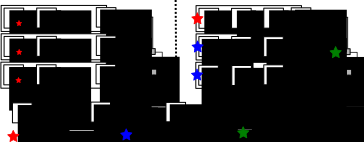
\includegraphics[width=0.95\textwidth]{fig/overview.png}
      %%
      \caption{~\todo{redo diagram to remove memory centric
      organization (it's a pipe dream)}
      Anatomy of a disaggregated rack. On the left a
      traditional rack with processors colocated with their memory
      interconnected by a switch. On the right is a high density
      disaggregated rack with processors separated from their memory
      by a top of rack switch. Stars mark locations for memory access
      serialization. Red denotes traditional processor centric
      serialization~\cite{memc3, cell, sonuma, storm, clover}, blue marks a
      memory centric architecture~\cite{aguilera2019designing}, and
      green marks a switch centric solution similar in spirit to
      proposed middle box solutions~\cite{254120}.
      \label{fig:overview}
      %%
      }
\end{figure*}



\section{Clover}

%%
Clover proposes that disaggregated data structures separate their
computational concerns into distinct responsibilities. Mainly memory
servers, which passively accept RDMA requests, Clients which issues read and
writes to the remote memory banks, and Metadata severs which
centralize and keep consistent the shared metadata of the disaggregated
data structures.

Through their experimentation they find that ideal throughput is
gained by placing client shared metadata out of datapath entirely, and
updating it opportunistically. Placing a metadata coordinator in the
datapath quickly leads to a performance bottleneck. Their algorithm
optimizes read operations, and allows for lockless line rate reads. In
the presence of writes however clovers operation throughput decreases
due to contention. When concurrent writes contest the same data a race
occurs in which the fastest writer wins. Write operations require two
messages, a data update (RDMA WRITE) and a check and set (RDMA CNS)
which updates old data to point to the new version. During this two
RTT operation any concurrent write to the same key will cause a
conflict. The slower writers will fail, and must retry their writes
after searching through clovers remote data structure for the next
write location to update their local cache (an operation known as
pointer chasing). On write heavy workloads these race conditions
happen frequently as illustrated in Figure~\ref{fig:conflicts}, which
leads to a sharp decrease in throughput.



%% what are we discussing
Clover's write strategy is opportunistic, it attempts to make updates
without acquiring locks, in the hope that no conflicts occur. When
they do occur it's just job of the writer to reconcile the conflict.
This opportunism amortizes the cost of lock acquisition when
contention is low, providing average case O(1) read/write and is used
in many high throughput concurrent data structures.

%%
We propose a middle ground between prior centralized approaches, and
clover's out of datapath metadata separation. Our insight is that by
caching small amount of a disaggregated data structures metadata in a
centralized location, write conflicts can be resolved at line rate in
the data path allowing for conflict free full read and write
throughput of disaggregated data structures. Using Clover as a
platform to prove our concept we design a lightweight middle box
algorithm which intercepts clovers RDMA read and write request, caches
a small amount (64 byte per key) amount of structural meta data and
resolves write conflicts by adjusting the destination RDMA address of
the writes. Our algorithm is implemented in DPDK, but is designed to
have low memory and computational overhead making it ideals for
network devices such as programmable switches and NICs.


%% The high level pitch about remote memory.
%Far memory projects typically have a remote CPU which is used to
%coordinate access to remote resources (cite all object systems). In a
%disaggregated system there is no remote CPU, therefore the coordination
%of reads and writes to remote locations must be done locally. For
%performance local caches of remote resources can be used to organize
%access to remote resources. For data structures which require
%consistency this creates a problem as stale caches can lead to data
%structure corruption.

\section{Our System}

Our system caches metadata for remote data structure on centralized
networking devices. Our prototype is implemented in DPDK, however our
algorithm could be implemented on a programmable switch or
programmable NIC as long as it sees all requests to remote memory. 
%% kinds of devices
A programmable TOR or our DPDK switch (which behaves as one) is ideal
for rack scale disaggregated structures that potentially span multiple
memory servers, while a programmable NIC implementation would be
limited limited to the memory server it is attached to. 

%%Technique example
The purpose of our technique is to resolve write conflicts to remote
memory. As an example of a conflict take a linked list implemented as
a remote data structure with a single operation, \textit{appendTail}.
This operation ensures that the next write to the data structure
writes to the tail of the linked list. This operation requires two
steps.  First a writer sends and RDMA write to the remote memory which
writes the data value for the new tail. After the data is written a
second operations consisting of an RDMA check and set (CNS) is issued
to the old tail which replaces it's NULL next pointer with the address
of the newly written tail.

This operation succeeds every time in the single threaded case as the
tail of the linked list is never moved by another process. Consider
instead the multi-threaded case in which two writer both attempt to
execute \textit{appendTail} concurrently. Both issue their first write
to remote memory successfully and then attempt to run an RDMA CNS on
the tail of the old list. This results in a race condition where one
process succeeds, and the other will fail. The process which executes
the CNS second fails because rather than finding a tail with a next
value of NULL, it finds the now penultimate member of the linked list
which now points to the value issued by the process which won the
race. 

The process which lost the race now needs to engage in \textit{Pointer
chasing}. It must iterative issue reads of the linked list until it
finds the location of the new tail. At which point it can reissue a
CNS to make the new tail point to it's value. This reconciliation
algorithm of pointer chasing must be run each time a conflict occurs.
For highly contested structures, the number of retries can grow
quickly, leading to large and unpredictable tail latencies.

In the case of clover this exact scenario occurs when key are write
contested. Their experiments with a zipf distribution on their keys
sees a \todo{5x} reduction in throughput.

%% What do we actually do
If a central arbiter where to observer the writes to this linked list
it would notice that the second CNS does not need to fail, it simply
needs to be redirected to point at the new tail of the list. 
%%
Our contention is that such a coordinator can be implemented in
network with minimal overheads to significantly improve the write
throughput. Using data structure specific information the coordinator
can cache recent writes, and steer concurrent ones to locations which
will result in successful operations and maintain the correctness of
the remote data structure.

In the case of clover we cache the tail of the linked list for each
key in clovers key value store. This results in an \textit{O(n)}
overhead where n is the number of keys. In our case for a key value
store consisting of 10k keys we need to store a key mapping and value
for each (both 64 bits) resulting in a total in network storage of
80KB. Note that this O(n) overhead is only a small fraction of clovers
metadata. Each key has a versioned history of writes, however only the
tail of the list is required to accelerate writes.

\textbf{Modifying RDMA in flight:}\sg{added long explicit explanation
about RDMA and conflict fixing} Interposing on an RDMA protocol is non
trivial. One solution (evaluated in as Clover
pDPM-central~\cite{clover}) would be to use an RDMA enabled middlebox
to setup connections between the clients and the memory servers which
would reissue RDMA request to the consistent locations. This solution
is impossible for a switch as it lacks the capabilities and resources
to establish RDMA connections. Further it has been demonstrated to be
a performance bottleneck. Our algorithm interposes on RDMA requests
transparently without storing any explicit RDMA state, or establishing
connections.

When RDMA write requests are issued our algorithm stores the locations
of the virtual addresses of the writes for each client thread. These
writes are marked as \textit{outstanding}. Outstanding writes are
writes which have been made to remote memory, but which have not yet
been made consistent in clover. Outstanding writes are not yet
connected to clovers key linked lists and therefore cannot be read by
other clients. Following an outstanding write clients will issue an
RDMA CNS which points the tail of the last committed write to the last
outstanding write the client issued, making it the new tail of the
list. Our algorithm detects the existence of a conflict when there is
more than one outstanding write for a given key. In addition to
tracking outstanding writes per client, our algorithm tracks the last
CNS issued to each key. This CNS marks the true tail of a keys linked
list. When a CNS for an outstanding write is seen, and the virtual
address of it's CNS points to an old tail, it's virtual address is
modified in flight (without the knowledge of the issuing client) to
point to the true tail of the list. The cached latest version of the
key is then updated to point to the address the CNS was directed to.
Clover clients learn the updated locations using their default read
algorithm.

RDMA packets are not intended to be modified in flight, and care must
be taken no to corrupt them. RDMA invariant CRCs are calculated at the
time of sending and are designed to ensure the integrity of the
payload. When CNS packets are modified their ICRC must be recalculated
or the modified packet will be rejected the RDMA hardware on the
receiving NIC. FPGA implementations of RDMA ICRC have been built in
the past~\cite{Mansour_2019}, the required CRC calculation is
identical to ethernet CRC, with the requirement of additional header
injection and field masking. We believe that this algorithm can be
implemented efficiently on a programmable switch.

\section{Evaluation}

Our experimental setup consists of 4 machines each with two sockets
equipped Intel Xeon E5-2640 CPU's and 265GB of main memory evenly
spread across two NUMA domains. Each machine has a Mellanox ConnectX-5
100Gbps NIC installed in a 16x PCIe slot. Each server is
interconnected via a 100Gbps Mellanox Onyx Switch. We designate a
single server to run as both the memory server (MS) and as the meta
data server (DN). Two machines are configured as clients, and a single
machine acts as a programmable switch.

All clover servers are configured using default routing settings.
Clients are configured to send directly to metadata and data servers.
We install OpenFlow rules on our Mellanox Onyx switch to redirect all
traffic to our DPDK packet switch.

\subsection{Conflict Resolution}

We test the performance gains of resolving write conflicts using our
middlebox solution. Clover clients are configured to run a YCSB-A
benchmark, 50\% read, 50\% write for 1 million requests. Request for
keys are distributed based on a zipf distribution generated with an
\textit{s} value of 0.75.\todo{show exactly what this means}. In each
experiment the number of client threads is increased which in turn
increases the load on the system. Clover request are blocking, and
thus the throughput is a factor of both the request latency and the
number of client threads. Figure~\ref{fig:throughput} shows the
performance gains by resolving write conflicts in flight.

As the number of clients increases so to does the probability that two
client threads will make concurrent writes to the same key. The number
of conflicts resolved in flight directly correlates to throughput
improvements as each successful request reduces the multiple round
trips necessary to resolve write conflicts. Our current implementation
provides a 1.42x throughput improvement at 64 client threads.

Our current experiments are limited by the scale of our experimental
setup, i.e more client machines can produce higher throughputs.
\todo{This is the speculation part we should cut}. 
The number of in flight conflicts is also effected by the zipf
distribution. We use a zipf of 0.75, however a zipf of 1.0 would
result in a distribution skewed towards fewer keys, which in turn
would result in higher conflicts. We found that Clovers current design
leads to high contention on ConnectX-5 NIC's as the number of RDMA
compare and swaps to the same memory region across different queue
pairs increases~\cite{design-guidelines}. In future work we plan to
both scale up the number of our client threads. Additionally our
design reduces the need for expensive compare and swap operations as
all cached keys have no conflicts. Our future implementations will
seek to reduce or eliminate CNS and replace them with low overhead
RDMA writes.

\begin{figure}
    \includegraphics[width=0.45\textwidth]{fig/throughput.pdf}
    \caption{Default Clover throughput vs Clover with write conflict
    detection and correction turned on.}
    \label{fig:throughput}
\end{figure}

\subsection{Memory Consumption}

Resources on networking hardware is scarce. High end SoC SmartNIC's
have just a few GB of RAM, and programmable switches have only MB's of
SRAM. Moreover the use of this memory is not free. Using memory for
any purpose other than buffer packets has a direct performance cost as
the number of packets which can be successfully buffered drops. Our
design takes the preciousness of memory in network into account. The
metadata we cache in network in the minimal necessary to resolve write
conflicts. While Clover's meta data consists of many MB of garbage
collection and version data we only cache the virtual address of the
last write per key. In addition we track the last key written per
client thread. Clients are not explicitly known to our middlebox and
are identified at runtime by their QP. Tracking clients in this way is
necessary to detect write conflicts in clover. This overhead could be
eliminated by explicitly adding key information to CNS requests.

Figure~\ref{fig:memory} Shows the memory overhead as a function of
keys. Note that 100K keys can be supported using 7\% of the available
memory on a Barefoot Tofino programmable switch (22MB).

\begin{figure}
    \includegraphics[width=0.45\textwidth]{fig/memory.pdf}
    \caption{Cost of caching metadata in network vs keyspace size.}
    \label{fig:memory}
\end{figure}

\subsection{Caching top \textit{N} keys} 
%%
Hot keys which are written frequently are the most likely to
contribute to conflict. Caching only hot keys results in relatively
large performance gains while requiring only a small portion of the
memory required to cache the entire keyspace. We test the effect of
caching only hot keys by restricting our in network cache to track and
resolve conflicts on only the top \textit{N} keys. In this experiment
RDMA requests for keys which are not caches pass through our middlebox
without modification, conflicts are resolved using Clovers
reconciliation protocol. We ran our experiment with 64 client threads,
with a total keyspace size of 1024 keys. Figure~\ref{fig:cache} shows
the relative throughput gains from caching the top N keys. The request
distribution is zipf(0.75), therefore the vast majority of conflicts
occur on the top 8 keys. The in network memory requirement for 8 keys
is 128 Bytes, which results in 1.3x throughput improvement.

\begin{figure}
    \includegraphics[width=0.45\textwidth]{fig/cache.pdf}
    \caption{Performance as a function of keys cached. Caching a few
    of the top n keys provides the greatest marginal throughput
    benefits.}
    \label{fig:cache}
\end{figure}

\section{Conclusion}

\todo{RDMA write contention}









\section{Discussion and future work}

Our approach only measures the benefits which clover observers by using our in
network contention resolution. However our approach is general, and in the
future we would like to add functionality for different systems. For example
Remote Regions~\cite{reigons} implements a POSIX file system API for remote
memory.  Our approach could also be used to remove contention here in a much
more standardized remote memory environment.

Clover represents a state of the art key value store for remote memory, however
it is designed with a different set of assumptions than we anticipate for future
systems. We believe that in the context of remote memory with programmable middle
boxes we should architect remote algorithms differently. Mainly that algorithms
and data structures should be designed with the assumption that conflicts can be
resolved using small amounts of high speed compute in network. We aim to explore
the design space of such algorithms and data structures in the future.

\section*{Acknowledgments}

\balance
\vspace{-0.3cm}
{\footnotesize \bibliographystyle{acm}
\bibliography{paper,sysnet}}
\vspace{-0.5cm}

\end{document}
